\documentclass[conference]{IEEEtran}
\IEEEoverridecommandlockouts
% The preceding line is only needed to identify funding in the first footnote. If that is unneeded, please comment it out.
\usepackage{cite}
\usepackage{amsmath,amssymb,amsfonts}
\usepackage{algorithmic}
\usepackage{graphicx}
\usepackage{textcomp}
\usepackage{xcolor}
\def\BibTeX{{\rm B\kern-.05em{\sc i\kern-.025em b}\kern-.08em
    T\kern-.1667em\lower.7ex\hbox{E}\kern-.125emX}}
\begin{document}

\title{Term Project Part-1 Report\\
{\footnotesize \textsuperscript{}}
\thanks{}
}

\author{\IEEEauthorblockN{Beyza BUTUN
\IEEEauthorblockA{2171411} \\
}

\IEEEauthorblockN{ Soner DURMAZ}
\IEEEauthorblockA{2171551 \\
}
}

\maketitle


\section{Introduction}
Before writing the code, we designed our project to receive an input in the form of a list, and to send it to the destination. To be able to do that,  we thought the source as the client which uses TCP, and we thought the broker as the server which uses TCP, and also as the client which uses UDP. So we combined these features in the code. Moreover, we thought that the routers are client and server which use UDP. Finally, we thought the destination as a server which uses UDP. After that, we started programming part.

\section{Programming Part}

\subsection{source.py}
First of all, we made the source take an input which are integers separated with comma. Then, we thought an algorithm to forward the input in the order of the one in the beginning.\\
To do that, first we calculated the number of integers which are the messages in the input, and we wrote a for loop to be able to deal with every message in the input separately. For every message, first we appended the number of integer in the input to the beginning of the message. Then, we appended the order of the message in the list. After that, we calculated time with a few functions from ntplib library, which is a open source libary and we downloaded it from internet to get syncronized time and we added it to the end of the message by packing it with struct.pack() function. The structure is like NumberofIntegers*Message$\&$theOrder+timePacked. Then, we created a client socket to send messages to the broker. Finally we sent them to the broker from this socket, and we closed the socket connection.

\subsection{broker.py}
Broker has to take message from the source, so it has to act like a server. To take the messages from source, first we created a server socket. Then, we received the messages from this socket. Broker also has to send messages to the routers. It means, It will act like a client. To reduce the loads of brokers, we decided to separate messages into two. We separated them in terms of their order in the list. We sent message in the odd order to the router1, and the other to the router2 after we created client socket. After we sent the messages to the routers, we closed the connection.

\subsection{router1.py - router2.py}
We forwarded odd order messages to the router1 and the others to the router2. To receive that messages, we created server socket for router1 and router2 respectively. Because routers don't change the messages, we only made them send the message to the destination by creating client socket. They sent messages to different destination IPs.

\subsection{destination.py}
Destination's aim is to receive messages from two routers, and combine them in terms of their order in the list. First we created two different server socket to receive messages from router1 and router2 respectively. To save the messages received, we defined a list called returnedList. And also, to save the end-to-end delays, we defined a list called statisticsList. After that, we defined a counter to count the number of received datas, and also we defined a boolean value to change receiving process between the router1 and router2. To receive the datas(messages), we created a loop, and we made the destination receive message from router1 and router2 respectively by changing the boolean value in this loop. After we received the message, we unpacked the time which we had appended to the end of the message by packing with struct.unpack() function. Then, we subtracted it from the time in that moment (we also get current time via the ntplib like we used in source.py), we calculated delay, and inserted it to the statistics list. \\
To be able to get the data itself and the count which represents the number of datas, we splitted it from '*','$\&$' and '+' characters. Then, we inserted the data to the returnedList. Its index in the returndList is the index in the given input. We checked if the data is the last or not. If it is, we printed the list, and we calculated average end to end delay to plot the graph. We also calculated the variance of end-to-end delay and error, but we commented them. \\
\\
\\
\\
\\
\\
\\
\\

\section{Graph}
To get the average and standard error of end-to-end delays we send a list of 100 integers (from 1 to 100) and get result with network emulation delay of 1ms +- 5ms, 20ms +- 5ms and 60ms +- 5ms. Then we plot the graph with following matlab code: \\
\begin{verbatim}
x=[1,20,60]; 
y=[11.9421482086,85.1922464371,245.569963455]; 
e=[0.809630671523,1.10141507557,1.08417912754]; 
errorbar(x,y,e); 
xlabel('Emulated Delay(ms)/+-5ms'); 
ylabel('End-to-End Delay(ms)');
title('Emulated Delay vs End-to-End Delay');
print('graph.png')
pause;
\end{verbatim}

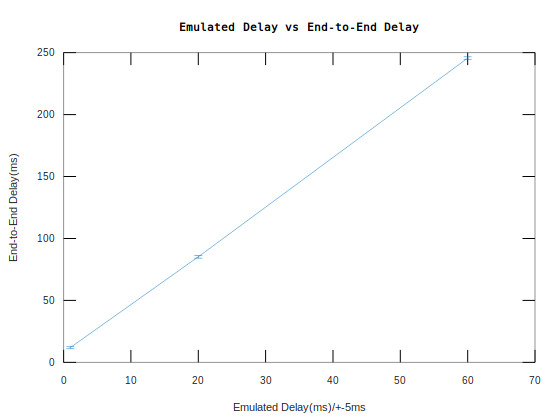
\includegraphics[width=9.5cm,scale=0.25]{graph.jpeg}\\[0.1cm]
\\
Our comment on graph, \\
At the beginning we expected to get a non-linear (due to 1ms emulated delays) graph because for 1ms emulated delay, the dominating factor is end-to-end delay's itself and for 20ms and 60ms emulated delays, the dominating factors are emulated delays, and so we expected to get two times emulated delay one for the link between broker and routers and the other one for the link between routers and destination. At the beginning of our test we get our expected graph even we didn't do anything about time synchronization but then suddenly our results regarding to statistical outputs of end-to-end delays became unstable. There were huge differences between results. To make results stable we took time from ntplib and we succeeded, but now averages are four times bigger than emulated delays and so the graph is nearly linear and 1ms delays nearly dominated the delays also. We think that the emulated delays affect both getting data and forwarding it to next node so 2*2=4 times of emulated delays.
\\
\\
\\
\textit{During the term project, we designed and implemented all parts together. }


\end{document}

